\section{Applications future}

Future applications will be highly compute-intensive, requiring efficient hardware and software components across various domains, including embedded systems, mobile devices, and data centers. 
Key characteristics of these future applications include:
\begin{itemize}
    \item \textit{Compute-intensiveness}: they will demand significant computational resources, necessitating optimized hardware and software regardless of their application domain.
    \item \textit{Connectivity}: these applications will be interconnected, either wired or wirelessly, and will often be online—globally interconnected through the Internet.
    \item \textit{Physical entanglement}: they will be embedded within and capable of interacting with the physical world, not only observing but also controlling their environment. 
        These systems will effectively merge into our everyday surroundings.
    \item \textit{Intelligence}: these applications will possess the capability to interpret noisy, incomplete, analog, or remote data from the physical world, allowing for smarter interactions and decision-making.
\end{itemize}
All major future applications will exhibit these traits to varying degrees. 
The ongoing integration of the digital and physical worlds (manifested through the Internet of Things (IoT) and Cyber-Physical Systems (CPS)) will be driven by advances in cognitive computing, big data analytics, and data mining.
\begin{figure}[H]
    \centering
    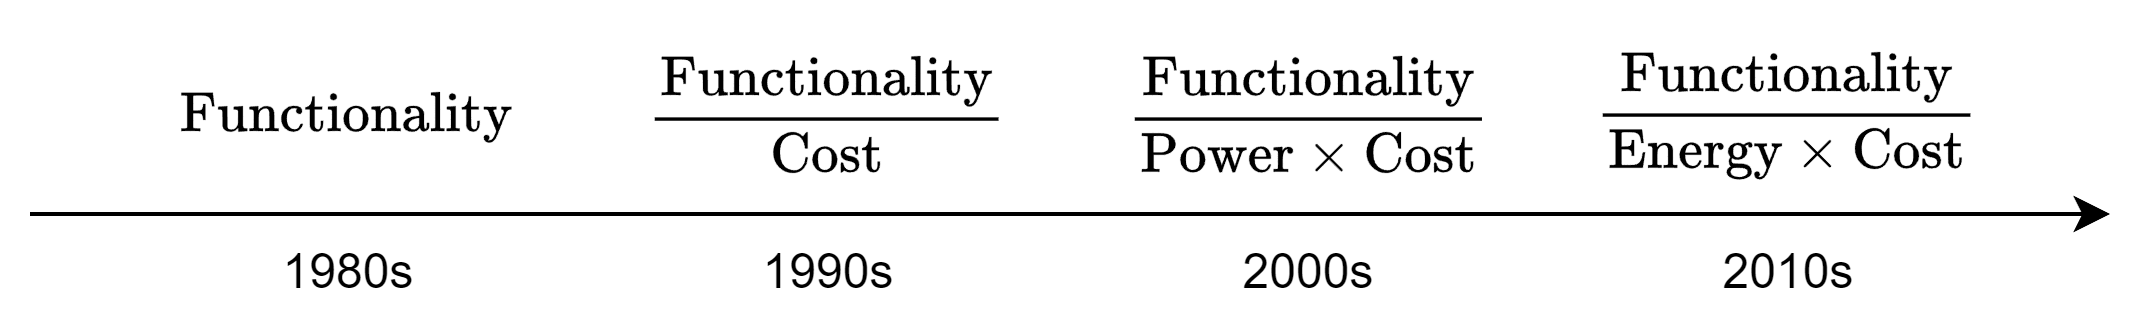
\includegraphics[width=0.75\linewidth]{images/time.png}
    \caption{Industry requirements}
\end{figure}
The challenge is that optimizing for functionality, energy, and cost remains difficult:
\[\dfrac{\text{functionality}}{\text{energy}\times\text{cost}}\]
However, successfully optimizing this metric often leads to improvements across simpler metrics as well.

While the number of transistors in modern systems can continue to increase, a key challenge is that we cannot power all of them simultaneously. 
This limitation drives the need for innovative approaches to using extra transistors more efficiently. 
Techniques like multicore and many-core processors, as well as domain-specific processors, are becoming essential. 
Additionally, heterogeneous processing combined with aggressive power management is crucial for optimizing performance across various tasks.
As data generation continues to accelerate it becomes increasingly important to ensure that computation is carried out in the most efficient location.
This efficiency is necessary to cope with the imbalance between the massive growth of data and the slowing progress of Moore's Law.

\subsection{Transistors and cores}
As transistors shrink in size, several challenges emerge. 
Process variation, physical failures, and aging mechanisms, such as negative bias temperature instability (NBTI), can degrade device performance over time. 
With very-large-scale integration (VLSI), packing more transistors into smaller spaces increases power density, which in turn creates thermal issues. 
Furthermore, traditional communication subsystems struggle to provide adequate power-performance trade-offs in these densely packed systems. 

For instance, Network-on-Chip (NoC) designs can consume up to 30\% of total chip power, and their performance plays a critical role in the efficiency of multicore architectures, which are increasingly necessary for improving system performance across various applications.

\subsection{Silicon challenges}
Despite silicon being a relatively good thermal conductor (about four times worse than copper), large chips can still experience significant temperature gradients, especially in high-performance CPUs. 
This creates hot spots that can affect chip reliability and performance. 
One practical solution involves dividing the chip into concentric rings and applying dynamic voltage and frequency scaling (DVFS) to each region. 
By fine-tuning voltage and frequency for each ring, it becomes possible to optimize performance while maintaining thermal balance, preventing excessive heat buildup in certain areas.

\subsection{Frequency scaling}
Modern systems address power management by partitioning chips into independent islands that operate at different voltage and frequency levels. 
This approach allows sections of the chip to be dynamically turned off when not in use, a process known as power gating. 
By adjusting power usage in this way, overall system energy efficiency is greatly improved without compromising performance when it is needed.

\subsection{Cooling systems}
Cooling systems are critical to managing the thermal output of modern computing hardware, and various methods are used depending on the specific requirements. 
Air cooling, while common, suffers from a low heat transfer coefficient (HTC), poor chip temperature uniformity, and requires large heat sinks and air ducts, particularly in data centers.
It is also noisy and expensive to maintain. Water cooling offers an improvement, with better HTC, more uniform chip temperatures, smaller heat sinks, and fewer fans. 
Water cooling also allows for potential heat recovery, though it requires large pumps to function effectively.

Two-phase cooling systems present an even more efficient solution. 
They provide higher HTC, better chip temperature uniformity, and smaller pumps, along with isothermal coolant, which helps maintain consistent temperatures across the chip. 
This method excels at cooling hot spots and also allows for heat recovery. However, two-phase cooling systems suffer from low pump efficiency and reliability issues.

New innovations, such as thermosyphon cooling, are emerging as promising alternatives, offering advanced methods to maintain chip performance while effectively managing heat dissipation.